\label{chap:results_discussions}
\section{Results}

During the internship, I have been able to understand Knowledge Acquisition, its role in improving 
a search engine, its pipeline components and to propose software architecture, different processing 
paradigms, and algorithms to implement them. Acquiring knowledge from a relational database of the 
company is the first process of IR improvement. It is also worth to mention that the software 
that I have been developing is going to be used once since all it does is to take the original 
database of the company and build two databases(i.e., one for storing KG and the other for semantic 
product descriptions).

Through an iterative process of acquiring more knowledge from either SMEs or the relational database, 
it is possible to improve the organic search quality as well. The developed program with a bit of 
modifications can be adjusted to integrate new knowledge more efficiently. Integrating new knowledge 
is also helpful to adjust our heuristics and build even more suitable ones. Analysing user queries and 
their activities is also helpful to understand the importance of different concepts and relations. 
Building an ontology and/or knowledge graph should be built upon the necessary and sufficient concepts 
and relations.

\subsection{Library}

As a result of different kinds of processes required for the knowledge acquisition, I have 
built a library to abstract away most of the low-level implementation details. One of the most 
important demands for this project is maintainability and readability. To achieve this goal, 
I have mainly focused on the clean software architecture as mentioned in the previous chapter. 
The library helps us to develop any high-level software application(s) on top of it. Since 
\textit{Python3+} has been chosen to be the main programming language, the library could be 
\textit{import}ed into a project to be used.

\begin{table}[H]
	\centering
	\begin{tabular}{|p{0.25\textwidth}|p{0.70\textwidth}|}
		\hline
		\textbf{Library} & \textbf{Used for} \\
		\hline
		\texttt{spacy} & NLP on user queries/model descriptions \\
		\hline
		\texttt{requests} & sending requests to databases \\
		\hline
		\texttt{threading} & parallization of ETL operations \\
		\hline
		\texttt{abc} & making top-level classes abstract and reinforcing developers to 
		implement abstract methods \\
		\hline
		\texttt{json} & json file operations \\
		\hline
		\texttt{logging} & logging \\
		\hline
		\texttt{configparser} & parsing ".ini" configuration files \\
		\hline
		\texttt{urllib.parse} & encoding IDs for OTTR \\
		\hline
	\end{tabular}
	\caption{External libraries}
	\label{tab:external_libraries}
\end{table}

\subsection{Command-Line Interface}

Several external libraries have been used in this project for different purposes. Two most important 
ones are \textit{spacy} and \textit{requests}. Instead of using the functionalities provided by these 
libraries directly, I have developed seperate classes that get rid of unnecessary and irrelevant 
functionalities and keep only the ones that are relevant to this project.

Spacy is a well-designed library used in industry for natural language processing. However, it has 
many functionalities that would be considered overhead for this project. Due to this reason, 
I have built a custom language model that is suitable for our needs.

Requests library helps developers to send/recieve information to/from endpoints. The send a request, 
request body, target url, method(i.e., GET, POST, etc.) have to be provided. Building scroll queries 
as described previously is necessary for abstraction of writing request bodies and/or target urls 
manually.

By using the devloped library and custom language model (see appendix \ref{prog:library}), a simple 
CLI\footnote{Command-Line Interface} has been developed. Both ETL-1 and ETL-2 processes 
can be run by the same program. All a user is required to do is to enter his/her choice of 
process after the prompt.

\subsection{Tests}

\paragraph{Invalid Configuration Handling.}
To execute ETL operations, one needs to provide the program a configuration. This configuration is 
recommended to be in the ".ini" file format, however, several environment variables can also be 
used. An example configuration file looks like in figure \ref{fig:config_example}. It is parsed and 
used by different operations such as Extractor and Loader (i.e., ESQuery).

\begin{figure}[H]
	\centering
	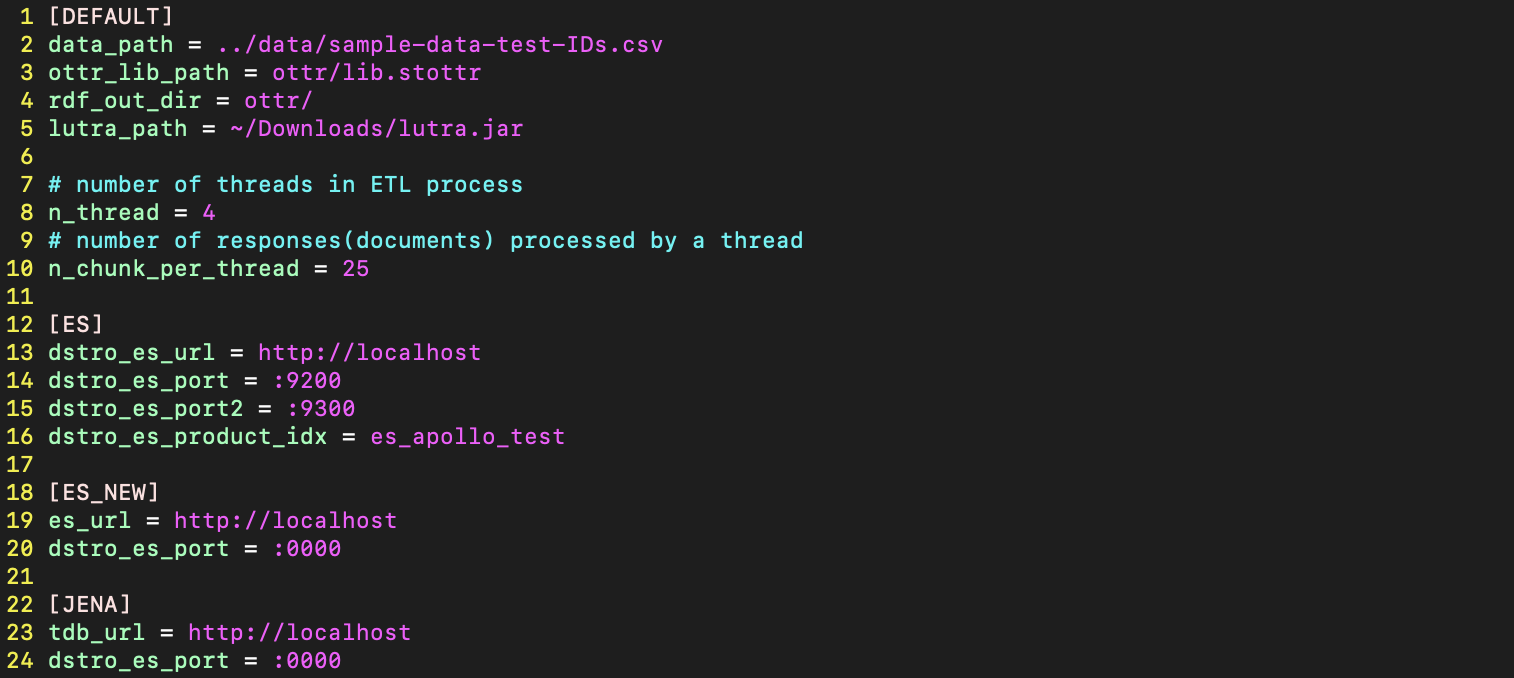
\includegraphics[width=0.75\textwidth]{../../resources/config_example.png}
	\caption{Configuration File example}
	\label{fig:config_example}
\end{figure}

The first four attributes can also be set with the help of environment variables. If neither 
environment variables are set nor configuration file misses some of the necessary attributes, 
program will halt with a self-descriptive error message.

\paragraph{Invalid Document Handling.}
As the extraction process of IDs have been implemented with 
\textit{regex}\footnote{Regular Expression} there are unittests to test edge cases. There are two 
cases: extracted ID is not a real ID or there is an ID which is not extracted. It is good to develop 
tests for each case.

\begin{table}[H]
	\centering
	\begin{tabular}{|p{0.45\textwidth}|p{0.45\textwidth}|}
		\hline
		\textbf{String} & \textbf{Is ID?} \\
		\hline
		10-23GGEZ-SHEESH & Yes \\
		\hline
		240V & Yes \\
		\hline
		10-23ggez-sheesh & No \\
		\hline
		800A & Yes \\
		\hline
		LCDAMOGUSRT34 & Yes \\
		\hline
	\end{tabular}
	\caption{Examples for ID verification}
	\label{tab:tests_id}
\end{table}

As shown in table \ref{tab:tests_id}, the first and the last strings are actual IDs whereas the third 
one is not. However, the second and the fourth strings are not real IDs either although our heuristic 
currently cannot classify such types correctly.

% \subsubsection{Performance}

% \begin{table}[H]
% 	\centering
% 	\begin{tabular}{|p{0.56\textwidth}|p{0.20\textwidth}|p{0.20\textwidth}|}
% 		\hline
% 		\textbf{Process} & \textbf{Run-time} & \textbf{Memory usage} \\
% 		\hline
% 		ESQuery (ETL-1 Extractor) & ? & ? \\
% 		\hline
% 		ES2TDB (ETL-1 Transformer) & ? & ? \\
% 		\hline
% 		TerminalOps (ETL-1 Loader) & ? & ? \\
% 		\hline
% 		Total (ETL-1) & ? & ? \\
% 		\hline
% 		\hline
% 		SPARQLQuery (ETL-2 Extractor) & ? & ? \\
% 		\hline
% 		TDB2ES (ETL-2 Transformer) & ? & ? \\
% 		\hline
% 		FileOps (ETL-2 Loader) & ? & ? \\
% 		\hline
% 		Total (ETL-2) & ? & ? \\
% 		\hline
% 	\end{tabular}
% 	\caption{Benchmark results for 100 documents}
% 	\label{tab:benchmark}
% \end{table}

\section{Discussion}

We can see that the developed software may still contain some bugs and terminate unexpectedly. This 
is due to several factors such as lack of unittests and edge cases given to the existing tests, 
poorly designed production and consumption of OperationalData objects, and imperfect heuristic 
implementation. In fact, the library and the software need to be improved furthermore. Several 
factors can be improved as shown below:

\begin{itemize}
	\item Heurictics can be added or modified according to SMEs knowledge
	\item More test cases for individual ETL operations can be added or even tests can be automated
	\item Data production and consumption can be handled with encapsulated furthermore
	\item Configuration file template can be structured more clearly
	\item Benchmarks can be designed to test the performance of each operation as well as the whole 
		to choose the best between different processing architectures
	\item etc.
\end{itemize}

We hope that the current software architecture, some core ideas about the pipeline components and 
processing paradigms and algorithms for them are not very far away from multiple future versions 
of the library and the software. Several modifications have to be made only on the implementational 
level and not on the architectural level.
